%!TEX root = ../thesis.tex
%*******************************************************************************
%****************************** Second Chapter *********************************
%*******************************************************************************

\chapter{Interactive and Interpretable ML}
\label{chapter2}

\graphicspath{{Chapter2/figs/}}

The Human Computer Interaction (HCI) field presents a great amount of resources that can lead the way towards better and more user-centric ML systems. For example, Holzinger \cite{Holzinger2016} argues that HCI can be of great benefit for supporting Knowledge Discovery (KDD), suggesting that Interactive ML systems can improve their outcomes by incorporating user feedback. In the same way, Dudley et al. \cite{Dudley2018} summarize the interaction elements that should be considered when designing Interactive ML systems, namely: \textbf{sample review}, \textbf{feedback assignment}, \textbf{model inspection} and \textbf{task overview}. Known strategies for implementing the first two elements are briefly described in Sections \ref{subsec:dimred} and \ref{subsec:al-vil}. To the best of our knowledge, although the \textbf{model inspection} and \textbf{task overview} interaction elements do not have the same level of development, some related works are presented in Section \ref{subsec:param-error}.

We argue that the \textbf{model inspection} element can be complemented by producing different kinds of interpretations about the model continuously refined thanks to \textbf{feedback assignment}. Model interpretation indicates the ability to provide explanations about their inner working which could help users understand their results. In addition, these additional components could support the \textbf{task overview} interface element because, as Doshi-Velez and Kim \cite{Doshi-Velez2017c} and Lipton \cite{Lipton2017TheInterpretability} explain, model interpretation is used to achieve other important requirements in user-centric ML systems such as trust, unbiasedness, privacy, reliability, robustness, causality, transferability, informativeness and usability. More details are discussed in Section \ref{sec:interpretableml}.

The rest of the paper explains the general characteristics and differences of classic ML versus more user-centric approaches. Then we proceed to summarize some of the main findings of the Interactive and Interpretable ML sub-fields, to conclude by describing some guidelines on how to design such user-centric ML systems.

%********************************** %First Section  **************************************
\section{Interactive ML} %Section - 2.1 
\label{section2.1}

Involving the user in the learning process is not a trivial task, and for a long time it has not been the concern of both KDD and ML fields. The Human-Computer Interaction (HCI) field, according to Holzinger \cite{Holzinger2013}, cares about human perception, cognition, intelligence, decision-making and interactive techniques of visualization. By merging these fields, many research opportunities emerge including the paradigm where algorithms can interact with agents (humans) and optimize their learning behavior through these interactions, as established by Holzinger \cite{Holzinger2016}. A more formal definition of Interactive ML is given by Dudley and Kristensson \cite{Dudley2018ALearning}: \textit{``... is a co-adaptive process, driven by the user, but inherently dynamic in nature as the model and user evolve together during training''}. 

As described by Fails and Olsen \cite{Fails2003}, classic ML generally has some assumptions which can be addressed through the use of Interactive ML, such as:

\begin{itemize}
\item The introduction of many features in the model can become noise and therefore affect its performance. An Interactive ML system should provide to user the ability to perform feature selection through a friendly interface and evaluate the change produced immediately.
\item There is not enough training data. Similar to feature selection, the user also must be able to perform labeling under consideration or by a systematic way and evaluate the change produced in the model performance. 
\item It is desirable that the system can adapt quickly to new training data. Avoid overfitting, addressed by strategies such as cross-validation, is one of the main concerns when designing ML systems. In the context of Interactive ML, the user can take decisions (e.g. labeling correction) in areas where decision frontier is more fuzzy. Active Learning and Visual Interactive Labeling, described in Section \ref{subsec:al-vil}, support this user activity. 
\end{itemize}

According to Fails and Olsen \cite{Fails2003}, an interface for Interactive ML must meet the following requirements: train very quickly, accommodate hundreds to thousands of features, perform feature selection and support tens to hundreds of thousands of training examples. From a more generalized perspective, Dudley and Kristensson \cite{Dudley2018} provide 4 interface elements to be considered while designing an Interactive ML system: \textbf{sample review}, \textbf{feedback assignment}, \textbf{model inspection} and \textbf{task overview}. A synthesis of Interactive ML scenario is shown in Figure \ref{fig:InteractiveML}, where the first three elements previously mentioned enable the direct user interaction with the data or the model. The \textbf{task overview} element is avoided because we considered is transversal to whole system and it is closely related to user and task context. 

\begin{figure}[ht]
 \centering
 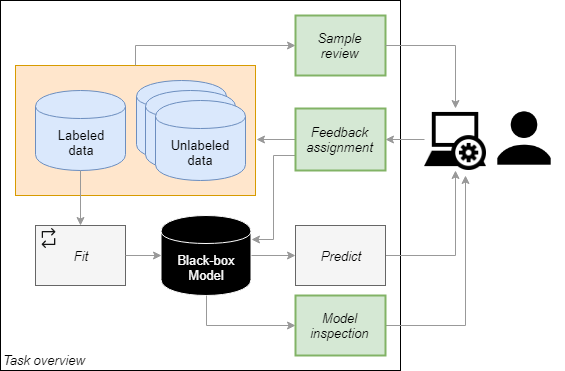
\includegraphics[width=0.45\textwidth]{InteractiveML.png}
 \caption{Interactive Machine Learning scenario. Three of four elements presented in Section \ref{sec:interactiveml} are highlighted, describing the direction of the interaction.}
 \label{fig:InteractiveML}
\end{figure}

Next subsections describe some related concepts to tackle the Interactive ML design process including some implementation scenarios. A more extensive revision about families of algorithms and application domains in the context of integrating ML and Visual Analytics can be found in Endert et al. \cite{Endert2017b}.

For \textbf{task overview}, no one relevant work was found in the context of Interactive ML because this interface element is closely related to the specific knowledge domain. Nevertheless, Dudley et al. \cite{Dudley2018} argue model accuracy and related metrics are not enough to evaluate the task fulfillment and this interface element should provide visibility of global objectives but also contextualize about other information such as availability of training data.

\subsection{Dimensionality Reduction}
\label{subsec:dimred}

In general terms, according to Tenenbaum et al. \cite{Tenenbaum2000} and Roweis and Saul \cite{Roweis2000}, Dimensionality Reduction (DR) deals with the problem of finding meaningful low-dimensional structures (compact representation) from high-dimensional data. For \textbf{sample review}, it is a valuable technique for representing high-dimensional data in principally two dimensions to validate the data distribution. A good DR representation can be one that allows evidence class separability, in the context of classification. Some algorithms for DR are PCA, t-SNE, proposed by Van der Maaten and Hinton \cite{VanDerMaaten2008VisualizingT-sne}, and UMAP, developed by McInnes and Healy \cite{McInnes2018UMAP:Reduction}.

In the context of clustering, Wenskovitch et al. \cite{Wenskovitch2018TowardsAnalytics} discuss about the combination of both techniques, contributing with a series of design challenges and questions from an extensive literature review. In the work of Wenskovitch and North \cite{Wenskovitch2017Observation-LevelAlgorithms}, data is projected by DR and a \textbf{feedback assignment} mechanism is provided to improve the cluster computation in an iterative way.

\subsection{Active Learning and Visual Interactive Labeling}
\label{subsec:al-vil}

One way of achieving \textbf{feedback assignment} is by leveraging users for labeling data. Active Learning (AL), described in Figure \ref{fig:AL}, consists of a series of analytical methods to select unlabeled data and present it to users in the form of queries for label assignment \cite{Holzinger2016}. Independently of the querying method used, the success of incorporating AL into an Interactive ML system lies on keeping the user labeling effort to a minimum. This can be achieved by only asking for feedback when the hope for a performance improvement given a specific query is high, as specified by Olsson \cite{Olsson2009} and Tong and Koller \cite{Tong2001}.

\begin{figure}[ht]
 \centering
 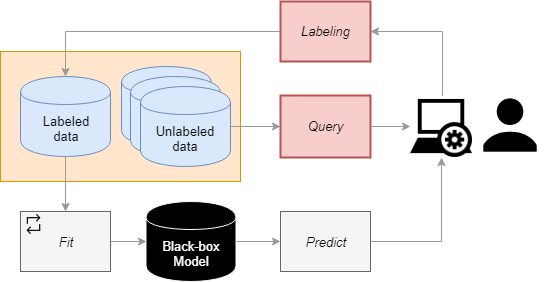
\includegraphics[width=0.45\textwidth]{AL.png}
 \caption{Active Learning scenario. An \textit{oracle}, typically a human, is asked for labels according to criteria based on maximization of performance improvement.}
 \label{fig:AL}
\end{figure}

Visual Interactive Labeling (VIL), in contrast to AL, delivers to user the selection of data candidates to be labeled. Nevertheless, user cognitive load can be reduced by incorporating visual techniques such as 2D Colormap, Class Coloring, Convex Hulls and Butterfly Plot, as described by Bernard et al. \cite{Bernard2018b}. AL and VIL are used in scenarios where there is small amount of labeled data, and where the domain knowledge from users can be useful to improve unreliable predictions. 

Complementing the work of Bernard et al. \cite{Bernard2018b}, they present a comparison among multiple VIL and AL strategies. The decision regarding to use either of the two methods depends highly on the user task complexity, the \textbf{sample review} technique and the class separability. In general terms, both techniques can compete to produce better and faster models.

\subsection{Parameter Tuning and Error Discovery}
\label{subsec:param-error}

Complementary to concepts previously described, we highlight two useful strategies to be included into an Interactive ML system: parameter tuning and error discovery. For the first strategy, we clarify that adjustment of model parameters does not imply necessarily to provide the ability to modify the number of hidden layers or link weights, talking about neural networks. The goal is to design interaction mechanisms usable for users even when these are not experts in ML. In other words, putting model parameters in terms of task domain, being this a non-trivial design decision. Some examples are described below.   

% Parameters
The work of Self et al. \cite{Self2016BridgingAnalytics} concludes with a list of user actions affecting implicitly the model parameters, consisting of: dragging points to form one or more new clusters, dragging an outlier into existing cluster, maximize one dimension weight and drag multiple sliders to equally large weights. In a similar way, Kapoor et al. \cite{Kapoor2010InteractiveClassification} focus on provide users the ability to refine the parameters of the confusion matrix according to their preferences and thus re-train the model in an iterative way.

% error discovery
An example of Interactive ML system for error discovery is presented by Chen et al. \cite{Chen2018b}. From a website classification problem, domain knowledge about the target class is introduced facilitating error discovery through semantic data exploration. While elements such as \textbf{sample review} and \textbf{model inspection} are introduced, an eventual desire of Interactive ML systems is missing: the ability to perform labeling correction and re-train the model to evaluate if it improves its performance.

% Learning by user knowledge
It is also important to highlight some works focused on implement systems that learn explicitly from user knowledge and not refining an specific algorithm proposed in literature. In Brown et al. \cite{Brown2012Dis-function:Interactively}, users are able to build the distance function for two dimensions data projection according to their own sense of distance. Chang et al. \cite{Chang2016AppGrouper:Results} propose a tool for clustering steered by user, having significantly higher quality than those from a pure algorithmic process.

%********************************** %Second Section  **************************************
\section{Interpretable ML} %Section - 2.2 
\label{section2.2}

In some scenarios, mechanisms to \textbf{sample review} and \textbf{feedback assignment} (e.g. user labeling or parameter tuning) may not be enough to successfully fulfill the user task. We argue \textbf{model inspection} implies opening the black-box model and presenting it to user in an interpretable or explainable way. In other words, \textbf{an Interactive ML system is not necessarily interpretable in terms of what model is learning and, in the opposite case, an Interpretable ML system could not involve all enough elements of interaction to perform the task in an usable and efficient way}. 

Nevertheless, the decision behind delivering interpretability to users must be careful studied, because as Doshi-Velez and Kim \cite{Doshi-Velez2017c} explain, interpretability is necessary and appropriate when there is an incompleteness in the problem formalization and can be avoided in these two scenarios: \textit{``(1) there are no significant consequences for unacceptable results or (2) the problem is sufficiently well-studied and validated in real applications that we trust the system’s decision, even if the system is not perfect''}.

Figure \ref{fig:interpretableML}, based on Hohman \cite{Hohman2018VisualFrontiers}, Doshi-Velez and Kim \cite{Doshi-Velez2017c} and Lipton \cite{Lipton2017TheInterpretability}, presents a condensed synthesis regarding to aspects to consider when thinking in produce interpretability. These aspects are grouped in six questions to be asked during the design process:

\begin{itemize}
    \item Why do you need to produce interpretability? Should the system be in the capacity to generate trust for predictions? Does it protect sensitive information in the data?.
    \item Who is the user of the system? Is the user a ML theoretical or a domain expert?
    \item What are the most important elements of the data or the model to visualize?
    \item How do you plan to represent those most important elements? Is it important for user to interact with those elements?
    \item When generate interpretations? Is the model under continuous refinement thanks \textbf{feedback assignment} or was the model previously trained and validated?
    \item Where will the system be deployed? Is the system intended to support a real-world problem in a company? Does the system contribute to produce scientific advances in a specific ML sub-field or any other knowledge domain?  
\end{itemize}

\begin{figure*}[ht]
 \centering
 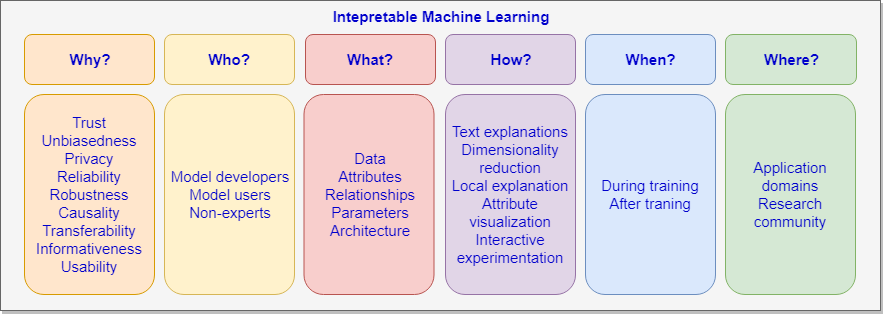
\includegraphics[width=0.9\textwidth]{InterpretableML.png}
 \caption{Aspects to consider when designing Interpretable ML systems. Based on Hohman \cite{Hohman2018VisualFrontiers}, Doshi-Velez and Kim \cite{Doshi-Velez2017c} and Lipton \cite{Lipton2017TheInterpretability}.}
 \label{fig:interpretableML}
\end{figure*}

Interpretable ML is not an isolated concept from Interactive ML, meaning that explanations could be produced in an interactive way to user considering the four interaction elements described in previous sections. Complementary, designers must not forget the system is constrained by an user task and users are those who are in the power to determine if the task was effectively fulfilled. User evaluations for interactivity and interpretability components, as in any HCI study, must be considered.

\subsection{Frameworks for Interpretability}

Ribeiro et al. \cite{Ribeiro2016} develop LIME. Based on local interpretability, this framework is able to explain predictions by learning an interpretable model locally around the prediction. The authors show the potential of the framework in applications based on tabular, image and text data. Complementary, LIME is extended by Teso and Kersting \cite{Teso2018WhyUsers} to explain the query produced in an AL scenario. Local explanations are the base of works focused on produce global interpretation as the case of the proposal by Yang et al. \cite{Yang2018GlobalPartitioning}. From contribution matrix representing the feature importance for every single data sample, product of frameworks such as LIME, a binary tree is learned to explicitly represent the most important decision rules that are implicitly contained in the black-box model. 

In Section 1, we mention that Deep Learning models have the disadvantage of being the least interpretable due to their large number of parameters. Contributions in this field have been achieved by producing interpretation of the features learned at each layer of a Neural Network, as demonstrated by Yosinski et al. \cite{Yosinski2015a} and Olah et al. \cite{Olah2018TheInterpretability}. A more extensive literature review about interpretability in Deep Learning can be found in Zhang and Zhu \cite{Zhang2018VisualSurvey}.

%********************************** %Third Section  **************************************
\section{The link between both worlds} %Section - 2.3
\label{section2.3}

